\chapter{二维共形不变性}

之前,我们关注全局的共形不变性,看到了 $d$ 维时空中场论的关联函数是如何被限制的。从现在起,我将详细解释本书的主题,二维共形场论。首先来解释二维共形场论特有的无穷维共形代数,关联函数满足的共形Ward恒等式,以及在共形场论中发挥巨大作用的算符乘积展开(OPE),这些共形场论的基本工具。

\section{初级场}
\subsection{准初级场}
考虑二维Euclid平面 $(x^0,x^1) $上的共形变换。引入复坐标 $z=x^0+ix^1 $,$ \bar{z}=x^0-ix^1 $,线元写成$ ds^2=dzd\bar{z}$ 。全局共形变换是 $(z,\bar{z}) $的$ S L(2, \mathbb{C}) \times S L(2, \mathbb{C})$ 变换,形如
\begin{equation}
z \rightarrow z^{\prime}=\frac{a z+b}{c z+d}, \quad \bar{z} \rightarrow \bar{z}^{\prime}=\frac{\bar{a} \bar{z}+\bar{b}}{\bar{c} \bar{z}+\bar{d}}
\end{equation}
该共形变换下,如果场$ \phi(z,\bar{z}) $变换为
\begin{equation}
		\phi^{\prime}\left(z^{\prime}, \bar{z}^{\prime}\right)=\left(\frac{d z^{\prime}}{d z}\right)^{-h}\left(\frac{d \bar{z}^{\prime}}{d \bar{z}}\right)^{-\bar{h}} \phi(z, \bar{z})
\end{equation}
称为\textbf{共形权是$ (h,\bar{h}) $的准初级场}。 $h=\bar{h} $时,变换 (3.2) 同上章共形维数是$ \Delta=h+\bar{h}$ 的准初级场定义中的一样。$ h\neq \bar{h}$ 时,二维旋转
\[
z^{\prime}=e^{i \theta} z, \quad \bar{z}^{\prime}=e^{-i \theta} \bar{z}
\]
下,准初级场 $\phi(z,\bar{z}) $变换为
\[
\phi^{\prime}\left(z^{\prime}, \bar{z}^{\prime}\right)=e^{-i \theta(h-\bar{h})} \phi(z, \bar{z})
\]
因此,差 $s=h-\bar{h}$ 表示\textbf{自旋}。

考虑共形权是 $(h_i,\bar{h}_i)$ 的准初级场$ \phi_i(z_i,\bar{z}_i) $( $i=1,\cdots,n $)的关联函数 $\left\langle\phi_{1}\left(z_{1}, \bar{z}_{1}\right) \cdots \phi_{n}\left(z_{n}, \bar{z}_{n}\right)\right\rangle $。全局共形变换 (3.1) 下,关联函数 $\left\langle\phi_{1}\left(z_{1}, \bar{z}_{1}\right) \cdots \phi_{n}\left(z_{n}, \bar{z}_{n}\right)\right\rangle$ 满足 (2.65) 的推广:
\begin{equation}
\left\langle\phi_{1}\left(z_{1}, \bar{z}_{1}\right) \cdots \phi_{n}\left(z_{n}, \bar{z}_{n}\right)\right\rangle=\left.\prod_{i=1}^{n}\left(\frac{\partial z^{\prime}}{\partial z}\right)^{h_{i}}\left(\frac{\partial \bar{z}^{\prime}}{\partial \bar{z}}\right)^{\bar{h}_{i}}\right|_{z=z_{i}, \bar{z}=\bar{z}_{i}}\left\langle\phi_{1}\left(z_{1}^{\prime}, \bar{z}_{1}^{\prime}\right) \cdots \phi_{n}\left(z_{n}^{\prime}, \bar{z}_{n}^{\prime}\right)\right\rangle
\end{equation}
准初级场的关联函数,两点和三点函数的形式可由全局共形不变性确定,除了有个未定常数。四点以上的关联函数如何依赖于交比,则无法这样确定。

\subsection{无穷小共形变换}

第1章讨论过,二维局域共形变换有无穷多个生成元。具有这一局域共形不变性的场论,称为\textbf{共形场论(CFT)}。共形场论最简单的例子,是无质量自由标量场和自由费米场。这些场是无相互作用的“自由”场, $N $点关联函数可由Wick定理计算。有相互作用的情形,从作用量根据Feynman规则微扰地计算关联函数会很困难。

为避免微扰计算中的发散问题,使用称为正则化的方法,但这时引入的截断参数具有长度量纲,明显破坏了标度不变性。更成问题的是,作用量本身也很难求出。有相互作用的共形场论,被认为描述重整化群的不动点,一般来说,不存在容许从自由场作用量作微扰展开的耦合常数。

考虑同时具有局域和全局共形不变性的情形,理论将受更多限制。事实上,我们将看到,无穷多个共形对称性,使我们能不用知道作用量,就确定关联函数。因此,要开始考察这样的理论,从理论的对称性(包括共形不变性)和对称性给出的关联函数满足的关系出发,而不是从作用量的具体形式,更加方便。在具有局域共形不变性的场论中,我们讨论从无穷小共形变换推出的Ward恒等式。

考虑二维中的相互作用场 $\varphi(x) $,作用量是$ S[\varphi]$ ,具体形式不必知道。在坐标$ x^\mu$ 的无穷小变换
\begin{equation}
x^{\mu} \rightarrow x^{\prime \mu}=x^{\mu}+\epsilon^{\mu}(x)
\end{equation}
下,场变为: $\varphi(x) \rightarrow \varphi^{\prime}(x)=\varphi(x)+\delta \varphi(x) $。假定作用量变为: $S \rightarrow S+\delta S$ 。作用量的这一无穷小变化 $\delta S$ 可写成
\begin{equation}
\delta S[\varphi]=\int d^{2} x T_{\mu \nu}(x) \partial^{\mu} \epsilon^{\nu}(x)
\end{equation}
$T_{\mu\nu}(x)$ 是能动张量。由Noether定理,Poincaré不变性给出 $T_{\mu\nu} $是守恒流,$ \partial^\mu T_{\mu\nu}=0$ 。无穷小Poincaré变换可写成 $\epsilon^{\mu}(x)=a^{\mu}+\epsilon^{\mu \nu} x_{\nu}$ 。这里, $a^\mu,\epsilon^{\mu\nu}$ 是无穷小参数,且 $\epsilon^{\mu\nu}$ 反对称。将这代入 (3.5) 可得,对平移变换,作用量的变化为零;如果对无穷小Lorentz变换,作用量的变化为零,需要满足$ T_{\mu\nu} $对称:
\begin{equation}
	T_{\mu \nu}=T_{\nu \mu}
\end{equation}

我们还要求作用量全局共形不变。如果无穷小标度变换 $\delta x^\mu=\alpha x^\mu $下不变,能动张量需要满足 $T^\mu_\mu=0 $(无迹条件)。可以看到,从$ T_{\mu\nu} $的两性质(对称和无迹条件),能推出特殊共形变换下的不变性。

\subsection{二维无穷小共形变换和初级场}

二维局域共形变换 $f(z)$ ,是 $z$ 的解析函数:
\begin{equation}
	z \rightarrow z^{\prime}=f(z), \quad \bar{z} \rightarrow \bar{z}^{\prime}=\bar{f}(\bar{z})
\end{equation}
在一般的共形变换下,按 (3.2) 变换的场,即
\begin{equation}
\phi^{\prime}\left(z^{\prime}, \bar{z}^{\prime}\right)=\left(\frac{d z^{\prime}}{d z}\right)^{-h}\left(\frac{d \bar{z}^{\prime}}{d \bar{z}}\right)^{-\bar{h}} \phi(z, \bar{z})
\end{equation}
称为\textbf{共形权是 $(h,\bar{h}) $的初级场}。因为变换 (3.7) 也包含全局共形变换,初级场是准初级场,但逆命题未必成立。在二维共形场论中,初级场的关联函数是研究主题之一。

考虑无穷小共形变换下初级场的行为。无穷小共形变换
\begin{equation}
z^{\prime}=z+\epsilon(z), \quad \bar{z}^{\prime}=\bar{z}+\bar{\epsilon}(\bar{z})
\end{equation}
下, (3.8) 成为
\begin{equation}
\phi^{\prime}(z+\epsilon(z), \bar{z}+\bar{\epsilon}(\bar{z}))=(1+\partial \epsilon(z))^{-h}(1+\bar{\partial} \bar{\epsilon}(\bar{z}))^{-\bar{h}} \phi(z, \bar{z})
\end{equation}
两边关于 $\epsilon,\bar{\epsilon}$ 展开,得到点 $(z,\bar{z}) $处场的无穷小变化是
\begin{equation}
\begin{aligned} \delta \phi(z, \bar{z}) & \equiv \phi^{\prime}(z, \bar{z})-\phi(z, \bar{z}) \\ &=-(\epsilon \partial+h \partial \epsilon+\bar{\epsilon} \bar{\partial}+\bar{h} \bar{\partial} \bar{\epsilon}) \phi(z, \bar{z}) \end{aligned}
\end{equation}

\section{无穷小共形Ward恒等式}

考虑全局共形变换的Ward恒等式 (3.3) 的无穷小版本。在无穷小变换 (3.9) 的情形, (3.3) 关于 $\epsilon$ 展开,可知关联函数满足微分方程
\begin{equation}
\sum_{i=1}^{n}\left(h_{i} \partial_{i} \epsilon\left(z_{i}\right)+\epsilon\left(z_{i}\right) \partial_{i}+\bar{h}_{i} \bar{\partial}_{i} \bar{\epsilon}\left(\bar{z}_{i}\right)+\bar{\epsilon}\left(\bar{z}_{i}\right) \bar{\partial}_{i}\right)\left\langle\phi_{1}\left(z_{1}, \bar{z}_{1}\right) \cdots \phi_{n}\left(z_{n}, \bar{z}_{n}\right)\right\rangle=0
\end{equation}
这里用了记号 $\partial_i\equiv \partial/\partial z_i$ , $\bar{\partial}_i\equiv \partial/\partial \bar{z}_i $。

第2章得到的关联函数形式,也可从微分方程 (3.12) 得到。全局共形变换,由无穷小变换
\begin{equation}
\epsilon(z)=\epsilon_{-1}+\epsilon_{0} z+\epsilon_{1} z^{2}, \quad \bar{\epsilon}(\bar{z})=\bar{\epsilon}_{-1}+\bar{\epsilon}_{0} \bar{z}+\bar{\epsilon}_{1} \bar{z}^{2}
\end{equation}
生成。对两点函数
\begin{equation}
G^{(2)}\left(z_{1}, z_{2}, \bar{z}_{1}, \bar{z}_{2}\right)=\left\langle\phi_{1}\left(z_{1}, \bar{z}_{1}\right) \phi_{2}\left(z_{2}, \bar{z}_{2}\right)\right\rangle
\end{equation}
考虑无穷小平移变换$ \epsilon(z)=\epsilon_{-1}, \bar{\epsilon}(\bar{z})=\bar{\epsilon}_{-1}$ ,我们有
\begin{equation}
\left(\partial_{1}+\partial_{2}\right) G^{(2)}\left(z_{1}, z_{2}, \bar{z}_{1}, \bar{z}_{2}\right)=\left(\bar{\partial}_{1}+\bar{\partial}_{2}\right) G^{(2)}\left(z_{1}, z_{2}, \bar{z}_{1}, \bar{z}_{2}\right)=0
\end{equation}
于是, $G^{(2)}$ 是 $z=z_1-z_2$ 和$ \bar{z}=\bar{z}_1-\bar{z}_2$ 的函数。接着考虑无穷小标度变换$ \epsilon(z)=\epsilon_{0} z$, $\bar{\epsilon}(\bar{z})=\bar{\epsilon}_{0} \bar{z}$ ,我们有
\begin{equation}
\begin{aligned} &\left(h_{1}+z_{1} \partial_{1}+h_{2}+z_{2} \partial_{2}\right) G^{(2)}\left(z_{1}, z_{2}, \bar{z}_{1}, \bar{z}_{2}\right) \\ =&\left(\bar{h}_{1}+\bar{z}_{1} \bar{\partial}_{1}+\bar{h}_{2}+\bar{z}_{2} \bar{\partial}_{2}\right) G^{(2)}\left(z_{1}, z_{2}, \bar{z}_{1}, \bar{z}_{2}\right)=0 \end{aligned}
\end{equation}
用 (3.15) 给出的$ \partial=\partial_{1}=-\partial_{2} $,关于 $z_i $的微分方程成为
\[
\left(h_{1}+h_{2}+z \partial\right) G^{(2)}=0
\]
解得$ G^{(2)} \sim z^{-h_{1}-h_{2}}$。再考虑反全纯部分,就得到两点函数是
\begin{equation}
G^{(2)}\left(z_{i}, \bar{z}_{i}\right)=\frac{C}{z^{h_{1}+h_{2}} \bar{z}^{\bar{h}_{1}+\bar{h}_{2}}}
\end{equation}

最后考虑无穷小特殊共形变换 $\epsilon(z)=\epsilon_{1} z^{2}, \bar{\epsilon}(\bar{z})=\bar{\epsilon}_{1} \bar{z}^{2} $,有微分方程
\begin{equation}
\begin{aligned} &\left(2 h_{1} z_{1}+z_{1}^{2} \partial_{1}+2 h_{2} z_{2}+z_{2}^{2} \partial_{2}\right) G^{(2)}\left(z_{1}, z_{2}, \bar{z}_{1}, \bar{z}_{2}\right) \\ =&\left(2 \bar{h}_{1} \bar{z}_{1}+\bar{z}_{1}^{2} \bar{\partial}_{1}+2 \bar{h}_{2} \bar{z}_{2}+\bar{z}_{2}^{2} \bar{\partial}_{2}\right) G^{(2)}\left(z_{1}, z_{2}, \bar{z}_{1}, \bar{z}_{2}\right)=0 \end{aligned}
\end{equation}
考虑全纯部分,首先用 $\partial=\partial_{1}=-\partial_{2} $,再代入 $G^{(2)}\left(z_{i}, \bar{z}_{i}\right)$ 的形式 (3.17) ,得到
\[
\left[2 h_{1} z_{1}+2 h_{2} z_{2}-\left(h_{1}+h_{2}\right)\left(z_{1}+z_{2}\right)\right] G^{(2)}=0
\]
这个式子要对任意 $z_1,z_2$ 成立,就应有 $2 h_{1}=h_{1}+h_{2}, 2 h_{2}=h_{1}+h_{2}$ ,也就是$ h_1=h_2$ 。反全纯部分也一样,那么两点函数就只在 $h_1=h_2 $时非零:
\begin{equation}
G^{(2)}\left(z_{i}, \bar{z}_{i}\right)=\left\{\begin{array}{cl} \frac{C_{h_{1}, h_{2}}}{\left(z_{1}-z_{2}\right)^{h_{1}+h_{2}}\left(\bar{z}_{1}-\bar{z}_{2}\right)^{\bar{h}_{1}+\bar{h}_{2}}}&, h_{1}=h_{2}, \bar{h}_{1}=\bar{h}_{2} \\ 0 &,其它情形 \end{array}
\right.\end{equation}
$h_i=\bar{h}_i $对应自旋为0的情形,我们复现了上章的结果。

对初级场的三点函数,同样有
\begin{equation}
\begin{aligned} &\left\langle\phi_{1}\left(z_{1}, \bar{z}_{1}\right) \phi_{2}\left(z_{2}, \bar{z}_{2}\right) \phi_{3}\left(z_{3}, \bar{z}_{3}\right)\right\rangle \\ =& \frac{C_{123}}{z_{12}^{h_{1}+h_{2}-h_{3}} z_{23}^{h_{2}+h_{3}-h_{1}} z_{13}^{h_{1}+h_{3}-h_{2}} \bar{z}_{12}^{\bar{h}_{1}+\bar{h}_{2}-\bar{h}_{3}} \bar{z}_{23}^{\bar{h}_{2}+\bar{h}_{3}-\bar{h}_{1}} \bar{z}_{13}^{\bar{h}_{1}+\bar{h}_{3}-\bar{h}_{2}}} \end{aligned}
\end{equation}
这里, $z_{ij}=z_i-z_j , C_{123} $是常数。

四点函数形如
\begin{equation}
\begin{aligned} &\left\langle\phi_{1}\left(z_{1}, \bar{z}_{1}\right) \phi_{2}\left(z_{2}, \bar{z}_{2}\right) \phi_{3}\left(z_{3}, \bar{z}_{3}\right) \phi_{4}\left(z_{4}, \bar{z}_{4}\right)\right\rangle \\ =& F\left(\frac{z_{12} z_{34}}{z_{13} z_{24}}, \frac{\bar{z}_{12} \bar{z}_{34}}{\bar{z}_{13} \bar{z}_{24}}\right) \prod_{i<j} z_{i j}^{-h_{i}-h_{j}+h / 3} \bar{z}_{i j}^{-\bar{h}_{i}-\bar{h}_{j}+\bar{h} / 3} \end{aligned}
\end{equation}
这里, $h=\sum_{i=1}^4h_i $, $\bar{h}=\sum_{i=1}^4\bar{h}_i $,$ z_{12}z_{34}/z_{13}z_{24} $是四点 $z_1,z_2,z_3,z_4 $的交比。

接下来推导一般局域共形变换的Ward恒等式。无穷小共形变换$ z \rightarrow z^{\prime}=z+\epsilon(z), \bar{z}\to\bar{z}^{\prime}=\bar{z}+\bar{\epsilon}(\bar{z}) $下,作用量变为: $S\to S+\delta S $。这里, $\delta S $由 (3.5) 给出。用复坐标 $(z,\bar{z}) $写成
\begin{equation}
\begin{aligned} \delta S &=\int d^{2} x\left(T_{z z} \partial^{z} \epsilon^{z}+T_{\bar{z} \bar{z}} \partial^{\bar{z}} \epsilon^{\bar{z}}\right) \\ &=\int d^{2} x\left(T_{z z} g^{z \bar{z}} \partial_{\bar{z}} \epsilon^{z}+T_{\bar{z} \bar{z}} g^{z \bar{z}} \partial_{z} \epsilon^{\bar{z}}\right) \end{aligned}
\end{equation}
复平面上 $g^{z\bar{z}}=2 $。初级场 $\phi(z,\bar{z})$ 在无穷小共形变换下,按 (3.11) 变换。

初级场$ \phi_i(z_i,\bar{z}_i) $的关联函数的路径积分形式是
\[
\left\langle\phi_{1}\left(z_{1}, \bar{z}_{1}\right) \cdots \phi_{n}\left(z_{n}, \bar{z}_{n}\right)\right\rangle=\int D \varphi \phi_{1}\left(z_{1}, \bar{z}_{1}\right) \cdots \phi_{n}\left(z_{n}, \bar{z}_{n}\right) e^{-S[\varphi]}
\]
$\varphi(z,\bar{z}) $是构成初级场 $\phi_i(z_i,\bar{z}_i) $的更基本的标量场。测度 $D\varphi $归一化了,以使右边系数为1。右边的积分变量可换成 $\varphi'$ :
\[
\left\langle\phi_{1}\left(z_{1}, \bar{z}_{1}\right) \cdots \phi_{n}\left(z_{n}, \bar{z}_{n}\right)\right\rangle=\int D \varphi^{\prime} \phi_{1}^{\prime}\left(z_{1}, \bar{z}_{1}\right) \cdots \phi_{n}^{\prime}\left(z_{n}, \bar{z}_{n}\right) e^{-S\left[\varphi^{\prime}\right]}
\]
假定场变化为$ \varphi',\phi_i' $,是由共形变换引起的,同时路径积分测度 $D\varphi $共形不变。代入 $S[\varphi']=S[\varphi]+\delta S$ ,得到
\[
\left\langle\phi_{1}\left(z_{1}, \bar{z}_{1}\right) \cdots \phi_{n}\left(z_{n}, \bar{z}_{n}\right)\right\rangle=\int D \varphi \phi_{1}^{\prime}\left(z_{1}, \bar{z}_{1}\right) \cdots \phi_{n}^{\prime}\left(z_{n}, \bar{z}_{n}\right) e^{-\delta S} e^{-S[\varphi]}
\]
代入 (3.22) 和初级场的无穷小变换$ \phi_{i}^{\prime}=\phi_{i}+\delta \phi_{i} $,保留到$ \epsilon $的一阶,得到
\begin{equation}
\sum_{i=1}^{n}\left\langle\phi_{1} \cdots \delta \phi_{i} \cdots \phi_{n}\right\rangle+\left\langle\int d^{2} x 2\left(T_{z z} \bar{\partial} \epsilon+T_{\bar{z} \bar{z}} \partial \bar{\epsilon}\right) \phi_{1} \cdots \phi_{n}\right\rangle=0
\end{equation}
这个式子称为\textbf{共形Ward恒等式}。

这里可用线积分的Green公式
\begin{equation}
\int_{C} P(x, y) d x+Q(x, y) d y=\int_{R} d x d y\left(\frac{\partial Q}{\partial x}-\frac{\partial P}{\partial y}\right)\quad \quad (3.24)
\end{equation}
这里,$ P(x,y),Q(x,y) $是 $(x,y)$ 的光滑函数。 $C$ 是平面上的Jordan闭合曲线,逆时针取向。 $R$ 是 $C $围成的区域,如图3.1。
\begin{figure}[h]
	\centering
	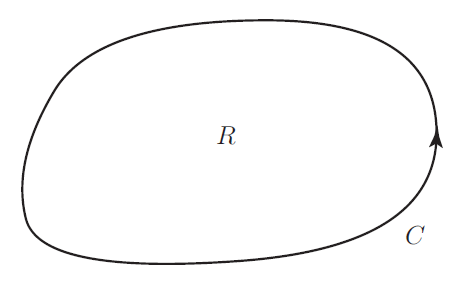
\includegraphics[width=0.6\linewidth]{fig/3.1.png}
	\caption{闭曲线$C$和它围成的区域$R$。}
\end{figure}

考虑用复坐标 $(z,\bar{z})$ 写,我们有
\begin{equation}
\begin{aligned} &d x=\frac{d z+d \bar{z}}{2},&&d y=\frac{d z-d \bar{z}}{2 i}\\ &\frac{\partial}{\partial x}=\partial+\bar{\partial}, && \frac{\partial}{\partial y}=i \partial-i \bar{\partial} 
\end{aligned}
\end{equation}
于是
\begin{equation}
	\int_{C} \frac{1}{2}(P-i Q) d z+\frac{1}{2}(P+i Q) d \bar{z}=\int_{R} d x d y(\partial(Q-i P)+\bar{\partial}(Q+i P))
\end{equation}
令
\[
T_{z z} \epsilon=Q+i P, \quad T_{\bar{z} \bar{z}} \bar{\epsilon}=Q-i P\]
得到
\begin{equation}
	\int_{R} d^{2} x\left\{\bar{\partial}\left(T_{z z} \epsilon\right)+\partial\left(T_{\bar{z} \bar{z}} \bar{\epsilon}\right)\right\}=\int_{C} \frac{T_{z z} \epsilon}{2 i} d z-\int_{C} \frac{T_{\bar{z} \bar{z}} \bar{\epsilon}}{2 i} d \bar{z}
\end{equation}
$T_{zz} $是全纯函数,$ T_{\bar{z} \bar{z}} $是反全纯函数,因此 (3.23) 改写成
\begin{equation}
\sum_{i=1}^{n}\left\langle\phi_{1} \cdots \delta \phi_{i} \cdots \phi_{n}\right\rangle+\left\langle\left(\int_{C} d z \frac{1}{i} \epsilon(z) T_{z z}-\int_{C} d \bar{z} \frac{1}{i} \bar{\epsilon}(\bar{z}) T_{\bar{z} \bar{z}}\right) \phi_{1} \cdots \phi_{n}\right\rangle=0 
\end{equation}
这里,积分路径 $C $围绕复平面上的 $z_1,\cdots,z_n $,如图3.2。
\begin{figure}[h]
	\centering
	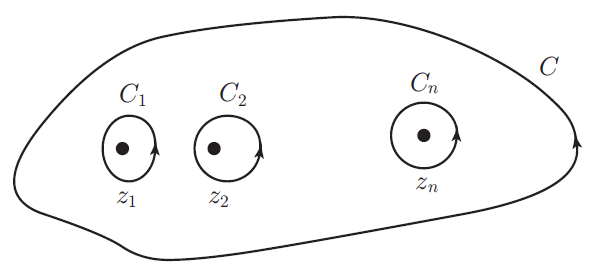
\includegraphics[width=0.6\linewidth]{fig/3.2.png}
	\caption{ 点$z_1,\cdots,z_n$,围绕它们的路径$C$,以及围绕各$z_i$的路径$C_i$。}
\end{figure}
定义 $T(z),\bar{T}(\bar{z}) $为
\[
2 \pi T_{z z}=T(z), \quad 2 \pi T_{\bar{z} \bar{z}}=\bar{T}(\bar{z})
\]
再代入初级场的无穷小变化, (3.28) 成为
\begin{equation}
\begin{aligned} &\int_{C} d z \frac{1}{2 \pi i} \epsilon(z)\left\langle T(z) \phi_{1} \cdots \phi_{n}\right\rangle-\int_{C} d \bar{z} \frac{1}{2 \pi i} \bar{\epsilon}(\bar{z})\left\langle\bar{T}(\bar{z}) \phi_{1} \cdots \phi_{n}\right\rangle\\ =&\sum_{i=1}^{n}\left(h_{i} \partial_{i} \epsilon\left(z_{i}\right)+\epsilon\left(z_{i}\right) \partial_{i}+\bar{h}_{i} \bar{\partial}_{i} \bar{\epsilon}\left(\bar{z}_{i}\right)+\bar{\epsilon}\left(\bar{z}_{i}\right) \bar{\partial}_{i}\right)\left\langle\phi_{1}\left(z_{1}, \bar{z}_{1}\right) \cdots \phi_{n}\left(z_{n}, \bar{z}_{n}\right)\right\rangle \end{aligned}
\end{equation}

这里,$ C$ 上对 $z$ 积分的被积函数,在 $C $围成的区域上是全纯的,除了插入初级场的点 $z_i$ 。根据积分路径的变形原理\footnote{[就是柯西定理]}, $C $上的积分等于围绕点 $z_i$ 的小回路 $C_i$ 上的积分之和,改写成
\[
\sum_{i=1}^{n} \int_{C_{i}} d z \frac{1}{2 \pi i} \epsilon(z)\left\langle T(z) \phi_{1} \cdots \phi_{n}\right\rangle
\]
对$ \bar{z}$ 的积分也可同样改写,那么期望值$ \langle \cdots \rangle$ 中,初级场的无穷小变化可写成
\begin{equation}
	\delta \phi_{i}\left(z_{i}, \bar{z}_{i}\right)=-\int_{C_{i}} d z \frac{1}{2 \pi i} \epsilon(z) T(z) \phi_{i}+\int_{C_{i}} d \bar{z} \frac{1}{2 \pi i} \bar{\epsilon}(\bar{z}) \bar{T}(\bar{z}) \phi_{i}
\end{equation}

因为$ C_i $可以任意小,贡献积分的只是能动张量位置 $z$ 趋于初级场位置 $z_i $时的奇异行为。具体来说,我们认为, $z\to z_i $时,期望值中可作如下展开:
\begin{equation}
T(z) \phi_{i}\left(z_{i}, \bar{z}_{i}\right)\sim\frac{h_{i}}{\left(z-z_{i}\right)^{2}} \phi_{i}\left(z_{i}, \bar{z}_{i}\right)+\frac{1}{z-z_{i}} \partial \phi_{i}\left(z_{i}, \bar{z}_{i}\right)+\text{Regular}
\end{equation}
“Regular”指展开中的常数项和$z-z_i $的正幂次项。右边在 $C_i $上积分,留数定理给出
\begin{equation}
\begin{aligned} &-\int_{C_{i}} \frac{d z}{2 \pi i} \epsilon(z)\left\{\frac{h_{i}}{\left(z-z_{i}\right)^{2}} \phi_{i}\left(z_{i}, \bar{z}_{i}\right)+\frac{1}{z-z_{i}} \partial \phi_{i}\left(z_{i}, \bar{z}_{i}\right)\right\} \\ =&-h_{i} \partial \epsilon\left(z_{i}\right) \phi_{i}\left(z_{i}, \bar{z}_{i}\right)-\epsilon\left(z_{i}\right) \partial \phi_{i}\left(z_{i}, \bar{z}_{i}\right) \end{aligned}
\end{equation}

这与初级场$ \phi(z,\bar{z}) $的无穷小变化 (3.11) 中依赖于 $\epsilon(z)$ 的项一致。依赖于 $\bar{\epsilon}(\bar{z})$ 的项也可同样得到:
\begin{equation}
\bar{T}(\bar{z}) \phi_{i}\left(z_{i}, \bar{z}_{i}\right) \sim \frac{\bar{h}_{i}}{\left(\bar{z}-\bar{z}_{i}\right)^{2}} \phi_{i}\left(z_{i}, \bar{z}_{i}\right)+\frac{1}{\bar{z}-\bar{z}_{i}} \bar{\partial} \phi_{i}\left(z_{i}, \bar{z}_{i}\right)+\text{Regular}
\end{equation}
这里的"Regular"也一样,指展开中的常数项和$ \bar{z}-\bar{z}_i $的正幂次项。

一般地,以算符之和的形式,描述算符 $A(z),B(w) $的乘积 $A(z)B(w)$ 在 $z\to w $时奇异行为的式子,称为 $A,B $的算符乘积展开(OPE)。 (3.31) 是 $T(z) $和初级场 $\phi_i(z_i,\bar{z}_i) $的OPE, $\epsilon(z)$ 代表任意无穷小共形变换。共形Ward恒等式 (3.30) ,除以 $\epsilon(z) $得到
\begin{align} 
	&\left\langle T(z) \phi_{1}\left(z_{1}, \bar{z}_{1}\right) \cdots \phi_{n}\left(z_{n}, \bar{z}_{n}\right)\right\rangle=\sum_{i=1}^{n}\left[\frac{h_{i}}{\left(z-z_{i}\right)^{2}}+\frac{1}{z-z_{i}} \partial_{i}\right]\left\langle\phi_{1}\left(z_{1}, \bar{z}_{1}\right) \cdots \phi_{n}\left(z_{n}, \bar{z}_{n}\right)\right\rangle  \\&\left\langle\bar{T}(\bar{z}) \phi_{1}\left(z_{1}, \bar{z}_{1}\right) \cdots \phi_{n}\left(z_{n}, \bar{z}_{n}\right)\right\rangle=\sum_{i=1}^{n}\left[\frac{\bar{h}_{i}}{\left(\bar{z}-\bar{z}_{i}\right)^{2}}+\frac{1}{\bar{z}-\bar{z}_{i}} \bar{\partial}_{i}\right]\left\langle\phi_{1}\left(z_{1}, \bar{z}_{1}\right) \cdots \phi_{n}\left(z_{n}, \bar{z}_{n}\right)\right\rangle
\end{align}

对全局共形变换 (3.13) ,Ward恒等式 (3.29) 的左边为零,那么初级场关联函数中加入$ T(z)$ 后,在 $z\to \infty$ 时,至少以 $z^{-4} $衰减。

\section{算符乘积和对易关系}

为更加详细地讨论局域共形对称性的Ward恒等式,我们考察二维场论中量子化与算符乘积展开的关系。

二维Euclid平面上,时间坐标是 $x^0 $,空间坐标是$ x^1$ ,引入复坐标
\begin{equation}
u=x^{0}+i x^{1}, \quad \bar{u}=x^{0}-i x^{1}
\end{equation}

令$ x^1 $有周期 $2\pi$ 。也就是说,空间是半径为 1 的圆, $(x^0,x^1) $是参数化圆柱的坐标。共形变换
\begin{equation}
	z=e^{u}, \quad \bar{z}=e^{\bar{u}}
\end{equation}

将圆柱映到复平面。无穷远过去 $x^0=-\infty$ 对应复平面原点$ z=0$ ,无穷远未来 $x^0=+\infty $对应无穷远点 $z=\infty$ 。时刻固定的圆,对应复平面上以原点为圆心的圆,时间流逝对应半径增大,如图3.3。
\begin{figure}[h]
	\centering
	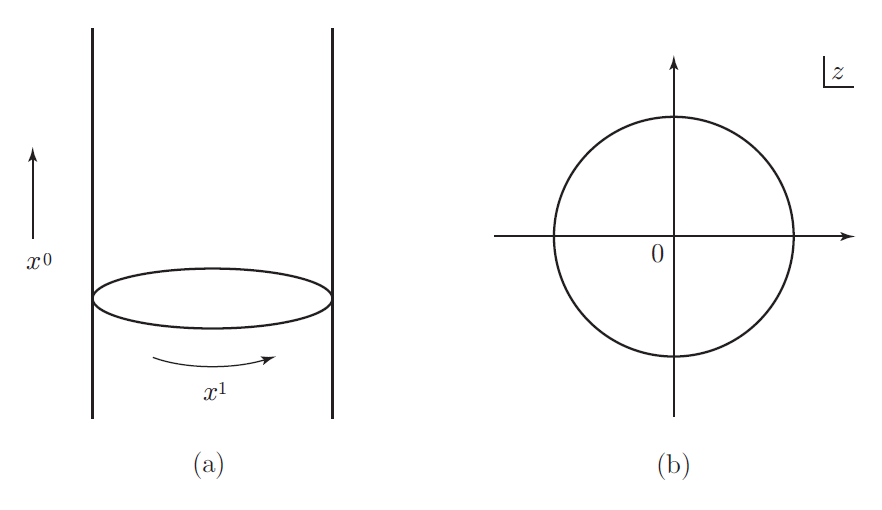
\includegraphics[width=0.6\linewidth]{fig/3.3.png}
	\caption{(a)圆柱上的坐标$(x^0,x^1)$,(b)复平面。}
\end{figure}

换句话说,时间在复平面上对应径向坐标。时间平移 $x^0\to x^0+a$ 对应复坐标 $z$ 的标度变换 $z\to e^a z$ ,空间平移 $x^1\to x^1+b$ 对应旋转 $z\to e^{ib}z $。

圆柱 $(x^0,x^1)$ 上场的期望值由编时乘积定义。在复平面上,自然就要按径向坐标排列场的顺序。这样的顺序称为\textbf{径向顺序},场的乘积称为\textbf{径向顺序积}。算符 $A(z),B(w) $的径向顺序积定义为
\begin{equation}
	R(A(z) B(w))=\left\{\begin{array}{ll} A(z) B(w), & |z|>|w| \\ B(w) A(z), & |z|<|w| \end{array}\right.
\end{equation}
复平面上共形场论中初级场的关联函数也可按径向顺序定义,接下来就展示这时得到的算符乘积与对易关系间自然的联系。

圆柱上算符$ A(x^0,x^1),B(x^0,y^1) $的等时对易关系 $[A(x^0,x^1),B(x^0,y^1)]$ ,对应复平面上的等径向坐标对易关系 $\left[A^{\prime}(z, \bar{z}), B^{\prime}(w, \bar{w})\right]$ , $|z|=|w| $。 $A'(z,\bar{z})$ 由$ A(x^0,x^1) $作共形变换 (3.37) 得到。

如果理论在特定的对称性下不变,由Noether定理,有守恒量 $J_\mu(x^0,x^1)$ ,$ \partial^\mu J_\mu=0 $。相应的守恒荷是
\begin{equation}
	Q=\int_{0}^{2 \pi} J_{0}\left(x^{0}, x^{1}\right) d x^{1}
\end{equation}
可以看到它是守恒的:
\begin{equation}
	\begin{aligned} \frac{d Q}{d x^{0}} &=\int_{0}^{2 \pi} \frac{\partial J_{0}\left(x^{0}, x^{1}\right)}{\partial x^{0}} d x^{1}=-\int_{0}^{2 \pi} \frac{\partial J_{1}\left(x^{0}, x^{1}\right)}{\partial x^{1}} d x^{1} \\ &=-J_{1}\left(x^{0}, 2 \pi\right)+J_{1}\left(x^{0}, 0\right)=0 \end{aligned}
\end{equation}
这里假定$ J_\mu(x^0,x^1)$ 满足周期性边界条件 $J_\mu(x^0,x^1+2\pi)=J_\mu(x^0,x^1) $。守恒荷生成无穷小变换,换句话说,场$ \phi$ 的无穷小变化 $\delta \phi $由对易关系给出: $\delta \phi=\epsilon[Q,\phi] $, $\epsilon $是无穷小参数。

二维无穷小共形变换对应流 $J_\mu=\epsilon^\nu T_{\mu\nu}$ ,守恒荷用复坐标 $(z,\bar{z}) $表达为
\begin{equation}
	Q=\int_{C_{0}} \frac{d z}{2 \pi i} \epsilon(z) T(z)+\int_{C_{0}} \frac{d \bar{z}}{2 \pi i} \bar{\epsilon}(\bar{z}) \bar{T}(\bar{z})
\end{equation}
这里, $C_0$ 是围绕原点的闭合曲线。

计算守恒荷与场的对易关系时,会出现同一点处场的乘积。因为这是发散的,需要先正规化计算出有限的量,再恢复正规化的参数。定义等时对易关系时,让时间发生微小的变化 $\epsilon $( $\epsilon $是正数)以正规化:
\[
\left[A\left(x^{0}, x^{1}\right), B\left(x^{0}, y^{1}\right)\right]= \lim _{\epsilon \rightarrow 0}\left(A\left(x^{0}+\epsilon, x^{1}\right) B\left(x^{0}, y^{1}\right)-B\left(x^{0}, y^{1}\right) A\left(x^{0}-\epsilon, x^{1}\right)\right)
\]
在复平面上,这样的操作对应
\begin{equation}
[A(z, \bar{z}), B(w, \bar{w})]=\lim _{|z| \rightarrow|w| \atop|z|>|w|} A(z, \bar{z}) B(w, \bar{w})-\lim _{|z| \rightarrow|w| \atop|w|>|z|} B(w, \bar{w}) A(z, \bar{z})
\end{equation}
换句话说,算符乘积被定义为总按径向顺序。

无穷小共形变换的生成元$ Q $与初级场 $\phi(w,\bar{w})$ 的对易关系,用径向顺序积写成
\begin{equation}
	\begin{aligned} \left[Q, \phi(w, \bar{w})\right]&=\int_{C_{1}} \frac{d z}{2 \pi i} \epsilon(z) T(z) \phi(w, \bar{w})-\int_{C_{2}} \frac{d z}{2 \pi i} \phi(w, \bar{w}) \epsilon(z) T(z)+\text{含}\bar{T}\text{的项}\\ &=\left(\int_{C_{1}} \frac{d z}{2 \pi i}-\int_{C_{2}} \frac{d z}{2 \pi i}\right) R(\epsilon(z) T(z) \phi(w, \bar{w}))+\text{含}\bar{T}\text{的项}\end{aligned}
\end{equation}
这里, $C_1 $是满足$ |z|>|w| $的围绕原点的闭合曲线, $C_2$ 则是满足 $|z|<|w| $。这两个积分的差,可转换成围绕 $z=w $的圆$ C_w$ 上的积分,如图3.4:
\begin{equation}
	[Q, \phi(w, \bar{w})]=\int_{C_{w}} \frac{d z}{2 \pi i} R(\epsilon(z) T(z) \phi(w, \bar{w}))+\text{含}\bar{T}\text{的项}
\end{equation}

\begin{figure}[h]
	\centering
	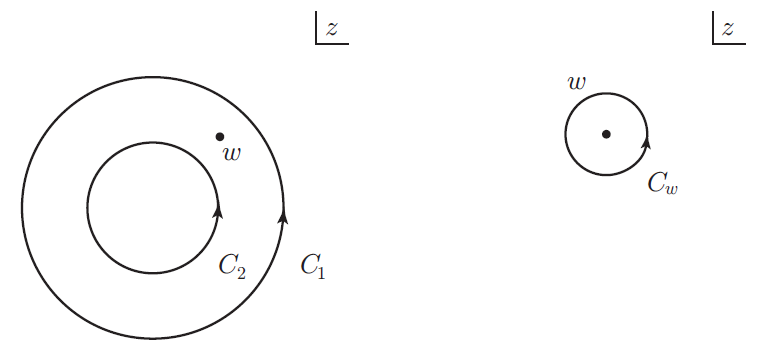
\includegraphics[width=0.6\linewidth]{fig/3.4}
	\caption{$C_1$:满足$|z| >|w|$的闭合曲线,$C_2$:满足$|z|<|w|$的闭合曲线,$C_w$:$C_1-C_2$变形得到的围绕$w$的闭合曲线。}
\end{figure}

因为$ C_w $可以任意小,贡献积分的是 $z\to w $,$T(z)$ 与$ \phi(w,\bar{w})$ 的OPE。代入OPE
\[
	T(z) \phi(w, \bar{w})=\frac{h}{(z-w)^{2}} \phi(w, \bar{w})+\frac{1}{z-w} \partial \phi(w, \bar{w})+\text{Regular}
\]
我们有
\begin{equation}
	\begin{aligned} \left[Q, \phi(w, \bar{w})\right]&=\int_{C_{w}} \frac{d z}{2 \pi i} \epsilon(z)\left\{\frac{h}{(z-w)^{2}} \phi_{i}(w, \bar{w})+\frac{1}{z-w} \partial \phi_{i}(w, \bar{w})\right\}+\text{含}\bar{T}\text{的项}\\ &=h \partial \epsilon(w) \phi(w, \bar{w})+\epsilon(w) \partial \phi(w, \bar{w})+\bar{h} \bar{\partial} \bar{\epsilon}(\bar{w}) \phi(w, \bar{w})+\bar{\epsilon}(\bar{w}) \bar{\partial} \phi(w, \bar{w}) \end{aligned}
\end{equation}
于是,通过$ {\color{red}-}\delta\phi=[Q,\phi] $得到了 $\phi$ 的无穷小变化\footnote{[按照本书的符号约定,似乎这里漏掉了一个负号,下一节也存在同样的问题,均使用红色标出]}。用径向顺序积定义的对易关系可由OPE计算。
\section{Virasoro代数}
\subsection{中心荷}
考虑能动张量 $T(z),\bar{T}(\bar{z})$ 的关联函数。因为能动张量 $T(z) $本来就是 $(2,0) $型张量,我们预期它是共形权为 $(2,0) $的初级场。同样, $\bar{T}(\bar{z})$ 是 $(0,2) $型张量,我们预期它是共形权为 $(0,2) $的初级场。$ T(z)$ 的单点函数 $\langle T(z)\rangle $平移不变,因此是不依赖于$ z$的常数,设为零:
\begin{equation}
	\langle T(z)\rangle=0, \quad\langle\bar{T}(\bar{z})\rangle=0
\end{equation}
全局共形不变性将$ T(z)$ 的两点函数限制成
\begin{equation}
	\langle T(z) T(w)\rangle=\frac{\frac{c}{2}}{(z-w)^{4}}, \quad\langle\bar{T}(\bar{z}) \bar{T}(\bar{w})\rangle=\frac{\frac{\bar{c}}{2}}{(\bar{z}-\bar{w})^{4}}
\end{equation}
这里, $c,\bar{c} $是常数。两点函数的形式 (3.47) 说明,$ T(z) $和$ T(w) $的OPE有 $z-w $的四阶极点,再由 $T(w) $本来就是$ (2,0)$ 型张量,得到OPE的形式是
\begin{equation}
	T(z) T(w)=\frac{\frac{c}{2}}{(z-w)^{4}}+\frac{2 T(w)}{(z-w)^{2}}+\frac{\partial T(w)}{z-w}+\cdots
\end{equation}

这里,$\cdots$代表展开中$ z-w $的非负幂次项。同样,$ \bar{T}(\bar{z})$ 和 $\bar{T}(\bar{w})$ 的OPE是
\begin{equation}
	\bar{T}(\bar{z}) \bar{T}(\bar{w})=\frac{\frac{\bar{c}}{2}}{(\bar{z}-\bar{w})^{4}}+\frac{2 \bar{T}(\bar{w})}{(\bar{z}-\bar{w})^{2}}+\frac{\partial \bar{T}(\bar{w})}{\bar{z}-\bar{w}}+\cdots
\end{equation}
常数 $c,\bar{c} $称为\textbf{中心荷}。

能动张量 $T(z) $的无穷小共形变化是
\begin{equation}
	{\color{red}-}\delta T(w)=\int \frac{d z}{2 \pi i} \epsilon(z) T(z) T(w)
\end{equation}
右边代入OPE (3.48) ,得到\footnote{$n$阶极点留数可以使用下式计算:\[\Res[f(z),a]=\lim_{z\to a}\frac{1}{(n-1)!}\frac{d^{n-1}}{dz^{n-1}}\left[(z-a)^nf(z)\right]\]}
\begin{equation}
	\begin{aligned} {\color{red}-}\delta T(w) &=\int \frac{d z}{2 \pi i} \epsilon(z)\left\{\frac{\frac{c}{2}}{(z-w)^{4}}+\frac{2 T(w)}{(z-w)^{2}}+\frac{\partial T(w)}{z-w}\right\} \\ &=\frac{c}{2} \frac{1}{3 !} \partial^{3} \epsilon(w)+2 \partial \epsilon(w) T(w)+\epsilon(w) \partial T(w) \end{aligned}
\end{equation}

能动张量 $T(w)$ 的无穷小共形变化,与初级场的不同只在于多了含$ \epsilon(w) $三阶导的项。在全局共形变换的情形, $\epsilon(w) $是$ w$ 的二次多项式,这项就为零。因此,全局共形变换下,$ T(w) $的行为同初级场一样,那么它是准初级场(见2.3节)。

有限共形变换 $z \rightarrow w=w(z) $下, $T(z) $变换为:\footnote{[此式对于一般的共形变换证明是较难的,但是对于无穷小变换可以很快地验证,本章末尾会对自由费米子和玻色子进行简要证明]}
\begin{equation}
	T(z) \rightarrow T^{\prime}(w)=T(z)\left(\frac{d w}{d z}\right)^{-2}-\frac{c}{12} S(w, z)\left(\frac{d w}{d z}\right)^{-2}
\end{equation}
$S(w,z)$ 是\textbf{Schwarz导数},定义为
\begin{equation}
	S(w, z)=\frac{\partial_{z} w \partial_{z}^{3} w-\frac{3}{2}\left(\partial_{z}^{2} w\right)^{2}}{\left(\partial_{z} w\right)^{2}}
\end{equation}

对全局 $SL(2,\mathbb{C})$ 变换$ w=(az+b)/(cz+d) $,有 $S(w,z)=0 $。同时,对共形变换 $f=f(z),w=w(f)$ 的复合 $w(f(z)) $,有
\begin{equation}
	S(w, z)=\left(\partial_{z} f\right)^{2} S(w, f)+S(f, z)
\end{equation}
中心荷出现在能动张量的两点函数中,导致能动张量的变换规则不同于常规的 $(2,0) $型张量。量子效应破坏守恒律和变换规则的现象,称为\textbf{反常}。 $c$ 就是表现\textbf{共形反常}的指标。

\subsection{ Virasoro代数}

将无穷小共形变换Laurent展开成:$\epsilon(z)=\sum_{n=-\infty}^{\infty} \epsilon_{n} z^{n+1}, \bar{\epsilon}(\bar{z})=\sum_{n=-\infty}^{\infty} \bar{\epsilon}_{n} \bar{z}^{n+1}\ (n\in \mathbb{Z}) $, $\epsilon_n,\bar{\epsilon}_n $对应的荷记作 $\epsilon_nL_n,\bar{\epsilon}_n\bar{L}_n $,那么$ L_n,\bar{L}_n\ (n\in \mathbb{Z})$ 是
\begin{equation}
	L_{n}=\oint \frac{d z}{2 \pi i} z^{n+1} T(z), \quad \bar{L}_{n}=\oint \frac{d \bar{z}}{2 \pi i} \bar{z}^{n+1} \bar{T}(\bar{z})
\end{equation}
这相当于 $T(z),\bar{T}(\bar{z}) $的Laurent展开
\begin{equation}
	T(z)=\sum_{n=-\infty}^{\infty} L_{n} z^{-n-2}, \quad \bar{T}(\bar{z})=\sum_{n=-\infty}^{\infty} \bar{L}_{n} \bar{z}^{-n-2}
\end{equation}
共形变换的荷可写成
\begin{equation}
	Q=\sum_{n=-\infty}^{\infty} \epsilon_{n} L_{n}+\bar{\epsilon}_{n} \bar{L}_{n}
\end{equation}

我们来计算$ L_n 和 L_m $( $n,m\in \mathbb{Z}$ )的对易子 $[L_n,L_m] $。先计算 $L_n $和 $T(w)$ 的对易关系,再围绕原点作积分 $\oint \frac{d w}{2 \pi i} w^{m+1}$ ,也就是
\begin{equation}
	\left[L_{n}, L_{m}\right]=\oint \frac{d w}{2 \pi i} w^{m+1} \int_{C_{w}} \frac{d z}{2 \pi i} z^{n+1} T(z) T(w)
\end{equation}
$C_w$ 是围绕$ z=w $的闭合曲线。右边代入OPE (3.48) :
\[
	\oint \frac{d w}{2 \pi i} w^{m+1} \int_{C_{w}} \frac{d z}{2 \pi i} z^{n+1}\left\{\frac{\frac{c}{2}}{(z-w)^{4}}+\frac{2 T(w)}{(z-w)^{2}}+\frac{\partial T(w)}{z-w}\right\}
\]
用留数定理计算对 $z$ 的积分,再根据$ L_n$ 的定义改写:
\begin{equation}
	\begin{aligned} &\oint \frac{d w}{2 \pi i} w^{m+1}\left\{\frac{c}{2} \frac{(n+1) n(n-1)}{3 !} w^{n-2}+2(n+1) T(w) w^{n}+\partial T(w) w^{n+1}\right\} \\ =&\frac{c}{12}(n+1) n(n-1) \delta_{n+m, 0}+2(n+1) L_{n+m}-(n+m+2) L_{n+m} \end{aligned}
\end{equation}
最后一项是这样算的:
\[
\oint \frac{d w}{2 \pi i} w^{m+n+2} \partial T(w)=\oint \frac{d w}{2 \pi i} \left[\partial\left(w^{m+n+2} T(w)\right)-(m+n+2) w^{m+n+1} T(w)\right]
\]
全导数不贡献积分。于是, $L_n,L_m$ 的对易关系是
\begin{equation}
	\left[L_{n}, L_{m}\right]=(n-m) L_{n+m}+\frac{c}{12} n\left(n^{2}-1\right) \delta_{n+m, 0}
\end{equation}

这个代数称为\textbf{Virasoro代数},$ L_n$ 是Virasoro代数的生成元。中心荷 $c$ 是常规的数,与Virasoro代数的生成元对易,这样的元素称为中心。因为右边也可看成$ L_n $和 $c$ 的线性组合,我们称这个代数是第1章讨论的二维共形代数加上$ c$ \textbf{扩张}得到的,是它的\textbf{中心扩张}。

$\bar{L}_n$ 也是同一代数的生成元:
\begin{equation}	
\left[\bar{L}_{n}, \bar{L}_{m}\right]=(n-m) \bar{L}_{n+m}+\frac{\bar{c}}{12} n\left(n^{2}-1\right) \delta_{n+m, 0}
\end{equation}
$T(z) $和 $\bar{T}(\bar{w}) $没有OPE,因此
\begin{equation}
\left[L_{n}, \bar{L}_{m}\right]=0	
\end{equation}
$L_{\pm 1},L_0 $生成全局共形变换,相应的代数中不出现 $c $,具体来说是
\begin{equation}
\left[L_{0}, L_{\pm 1}\right]=\mp L_{\pm 1}, \quad\left[L_{1}, L_{-1}\right]=2 L_{0}
\end{equation}
这个代数是 $\mathfrak{sl}(2,\mathbb{C})$ 。

\subsection{CFT的Hilbert空间}
我们来考察共形场论的Hilbert空间与Virasoro代数的表示间的关系。将初级场的关联函数表示成场算符乘积的真空期望值:
\begin{equation}
	\left\langle\phi_{1}\left(z_{1}, \bar{z}_{1}\right) \cdots \phi_{N}\left(z_{N}, \bar{z}_{N}\right)\right\rangle=\left\langle 0\left|R\left(\phi_{1}\left(z_{1}, \bar{z}_{1}\right) \cdots \phi_{N}\left(z_{N}, \bar{z}_{N}\right)\right)\right| 0\right\rangle
\end{equation}
$|0\rangle$ 是对应真空的右矢。关联函数在全局共形变换下不变。无穷小Ward恒等式是
\begin{equation}
	\begin{aligned} 0 &=\sum_{j=1}^{N}\left\langle\phi_{1}\left(z_{1}, \bar{z}_{1}\right) \cdots \delta \phi_{j}\left(z_{j}, \bar{z}_{j}\right) \cdots \phi_{N}\left(z_{N}, \bar{z}_{N}\right)\right\rangle \\ &=\sum_{j=1}^{N}\left\langle 0\left|R\left(\phi_{1}\left(z_{1}, \bar{z}_{1}\right) \cdots\left[Q, \phi_{j}\left(z_{j}, \bar{z}_{j}\right)\right] \cdots \phi_{N}\left(z_{N}, \bar{z}_{N}\right)\right)\right| 0\right\rangle \end{aligned}
\end{equation}
这里, $Q=\epsilon_{-1} L_{-1}+\epsilon_{0} L_{0}+\epsilon_{1} L_{1}$ 。右边也可写成
\[
	\left\langle 0\left|\left[Q, \phi_{1}\left(z_{1}, \bar{z}_{1}\right) \cdots \phi_{N}\left(z_{N}, \bar{z}_{N}\right)\right]\right| 0\right\rangle
\]
这要对任意 $\epsilon_{\pm1},\epsilon_0$ 成立,真空右矢 $|0\rangle $和左矢 $\langle 0|$ 就要在$ m=0,\pm 1$ 时满足
\begin{equation}
	L_{m}|0\rangle=0, \quad\langle 0| L_{m}=0
\end{equation}
这意味着真空是 $SL(2,\mathbb{C}) $不变的。

Virasoro代数的一般生成元$ L_m $作用在 $|0\rangle $上需要满足的条件,由 $T(z)|0\rangle $在 $z\to 0 $时正规来确定。根据 $T(z)$ 的Laurent展开式
\begin{equation}
	T(z)|0\rangle=\sum_{n=-\infty}^{\infty} L_{n}|0\rangle z^{-n-2}
\end{equation}
可以知道, $z\to 0$ 时不出现奇异性要求
\begin{equation}
	L_{n}|0\rangle=0, \quad n \geq-1
\end{equation}
对真空左矢$ \langle 0| $,则是 $\langle 0|T(z)$ 在 $z\to \infty $时正规,这要求\footnote{要看到这点,在$z \to \infty$处改用坐标$w = 1/z$。能动张量的变换规则给出$T(z) = \left( \frac{\partial w}{\partial z} \right)^2 T'(w)=w^4 T'(w)$。于是我们要求$\langle 0 | T'(w) = \langle 0 | z^4 T(z)$在$z \to \infty$时正规。}
\begin{equation}
	0=\langle 0| L_{n}, \quad n \leq 1
\end{equation}
用这个性质可以计算$ T(z) $的两点函数$ \langle T(z)T(w)\rangle $。$ |z|>|w|$ 时,由 (3.68),(3.69) 有
\begin{equation*}
	\begin{aligned} \langle 0|T(z) T(w)| 0\rangle &=\sum_{n=-\infty}^{\infty} \sum_{m=-\infty}^{\infty} z^{-n-2} w^{-m-2}\left\langle 0\left|L_{n} L_{m}\right| 0\right\rangle \\ &=\sum_{n=0}^{\infty} \sum_{m=-\infty}^{-2} z^{-n-2} w^{-m-2}\left\langle 0\left|L_{n} L_{m}\right| 0\right\rangle \end{aligned}
\end{equation*}
右边代入Virasoro代数 (3.60) 得到
\begin{equation*}
\begin{aligned} & \sum_{n=0}^{\infty} \sum_{m=-\infty}^{-2} z^{-n-2} w^{-m-2}\left\langle 0\left|\left(L_{m} L_{n}+\left[L_{n}, L_{m}\right]\right)\right| 0\right\rangle \\ =& \sum_{n=0}^{\infty} \sum_{m=-\infty}^{-2} z^{-n-2} w^{-m-2}\left\langle 0\left|\left\{(n-m) L_{n+m}+\frac{c}{12} n\left(n^{2}-1\right) \delta_{n+m, 0}\right\}\right| 0\right\rangle \\ =& \sum_{n=0}^{\infty} \frac{c}{12} n\left(n^{2}-1\right) \frac{1}{z^{2} w^{2}}\left(\frac{w}{z}\right)^{n} \\ =& \frac{\frac{c}{2}}{(z-w)^{4}} \end{aligned}
\end{equation*}
这复现了OPE的结果。

\subsection{BPZ共轭}
CFT的Hilbert空间上定义有自然的Hermite共轭(BPZ共轭)。它是将二维Minkowski时空中的Hermite共轭推广到Euclid空间得到的。

首先,定义作用在Hilbert空间上的算符的共轭。考虑Minkowski时空 $(t,x) $中的场 $A(t,x) $。时间演化由Hamiltonian生成, $t $时刻的场与 $t=0 $时的关系是
$$
A(t, x)=e^{i H t} A(0, x) e^{-i H t}
$$
这个关系式的Hermite共轭是
$$
A(t, x)^{\dagger}=e^{i H t} A(0, x)^{\dagger} e^{-i H t}
$$
也就是说,时间演化后作Hermite共轭,等价于 $t=0$ 时取Hermite共轭再时间演化。

时间 $t$ 解析延拓( $\tau=+i t$ )到虚轴\footnote{[原书为$\tau=-i t$]},就得到Euclid空间 $(\tau,x)$ 中的时间演化:
$$
A(\tau, x)=e^{H \tau} A(0, x) e^{-H \tau}
$$
这个关系式的Hermite共轭是
$$
A(\tau, x)^{\dagger}=e^{-H \tau} A(0, x)^{\dagger} e^{H \tau}
$$
也就是说,时间演化后作Hermite共轭,不同于 $\tau=0 $时取Hermite共轭再时间演化,还需要加上时间反演 $\tau \to -\tau$ 。我们将这个复合变换定义为Euclid空间中的“Hermite”共轭,本节用$ {}^+ $表示:
$$
A(\tau, x)^{+}=e^{H \tau} A(0, x)^{+} e^{-H \tau}
$$
在圆柱 $(x^0,x^1) $上定义共形权是 $(h,\bar{h}) $的初级场 $\phi'(u,\bar{u})$ ,它的“Hermite”共轭是
$$
\phi^{\prime}(u, \bar{u})^{+}=\phi^{\prime}(-\bar{u},-u)
$$
这里,$ u=x^{0}+i x^{1}, \bar{u}=x^{0}-i x^{1} $。通过共形变换 $z=e^{u}, \bar{z}=e^{\bar{u}} $,将$ \phi'(u,\bar{u})$ 映到复平面上,得到的初级场记作 $\phi(z,\bar{z}) $,它与$ \phi'(u,\bar{u})$ 的关系是
$$
\phi(z, \bar{z})=\left(\frac{d z}{d u}\right)^{-h}\left(\frac{d \bar{z}}{d \bar{u}}\right)^{-\bar{h}} \phi^{\prime}(u, \bar{u})
$$
由 $dz/du=z,d\bar{z}/d\bar{u}=\bar{z} $得到
\begin{equation}
	\phi(z, \bar{z})=z^{-h} \bar{z}^{-\bar{h}} \phi^{\prime}(u, \bar{u})
\end{equation}
那么 $\phi(z,\bar{z}) $的“Hermite”共轭是
$$
\phi(z, \bar{z})^{+}=\bar{z}^{-h} z^{-\bar{h}} \phi^{\prime}(u, \bar{u})^{+}
$$
另一方面, $(u,\bar{u}) $时间反演成$ (-\bar{u},-u)$ 后,$ (z,\bar{z}) $就会变成 $(1/\bar{z},1/z)$ ,因此 (3.70) 时间反演后成为
$$
\phi\left(\frac{1}{\bar{z}}, \frac{1}{z}\right)=\left(\frac{1}{\bar{z}}\right)^{-h}\left(\frac{1}{z}\right)^{-\bar{h}} \phi^{\prime}(-\bar{u}, -u)
$$
于是有
\begin{equation}
	\phi(z, \bar{z})^{+}=\bar{z}^{-2 h} z^{-2 \bar{h}} \phi\left(\frac{1}{\bar{z}}, \frac{1}{z}\right)
\end{equation}
同时,初级场 $\phi(z,\bar{z}) $在 $w=1/z $变换下成为
\begin{equation}
\begin{aligned} \tilde{\phi}(w, \bar{w}) &=\left(\frac{d w}{d z}\right)^{-h}\left(\frac{d \bar{w}}{d \bar{z}}\right)^{-\bar{h}} \phi(z, \bar{z}) \\ &=\left(-w^{2}\right)^{-h}\left(-\bar{w}^{2}\right)^{-\bar{h}} \phi\left(\frac{1}{w}, \frac{1}{\bar{w}}\right) \end{aligned}
\end{equation}
与 (3.71) 比对得到
\begin{equation}
	\phi(z, \bar{z})^{+}=(-1)^{h+\bar{h}} \tilde{\phi}(\bar{z}, z)
\end{equation}
因为能动张量 $T(z)$ 的共形权是 $(2,0) $, (3.71) 给出
\begin{equation}
	T(z)^{+}=T\left(\frac{1}{\bar{z}}\right) \frac{1}{\bar{z}^{4}}
\end{equation}
代入 $T(z)$ 的Laurent展开 (3.56) ,得到
$$
\sum_{m=-\infty}^{\infty} L_{m}^{+} \bar{z}^{-m-2}=\bar{z}^{-4} \sum_{n=-\infty}^{\infty} L_{n} \bar{z}^{n+2}
$$
从而
\begin{equation}
	L_n^+=L_{-n}
\end{equation}

CFT Hilbert空间中态矢 $|\phi\rangle$的BPZ共轭按如下方式定义:首先, $SL(2,\mathbb{C}) $不变真空$ |0\rangle$ 的BPZ共轭是$ \langle 0|$ :
$$
(|0\rangle)^{+}=\langle 0|
$$
初级场 $\phi(z,\bar{z}) $对应的态矢 $|\phi\rangle$ 定义为
\begin{equation}
	|\phi\rangle=\lim _{z, \bar{z} \rightarrow 0} \phi(z, \bar{z})|0\rangle
\end{equation}
$z=\bar{z}=0 $对应无穷远过去 $x^0\to -\infty$ 。态 $|\phi\rangle$ 的BPZ共轭,定义为无穷远未来 $z\to\infty $( $x^0\to +\infty $)时的态
\begin{equation}
	\langle\phi|=\lim _{w, \bar{w} \rightarrow 0}\langle 0| \tilde{\phi}(w, \bar{w})(-1)^{h+\bar{h}}=\lim _{z, \bar{z} \rightarrow \infty}\langle 0| \phi(z, \bar{z}) z^{2 h} \bar{z}^{2 \bar{h}}
\end{equation}
$z\to \infty$ 就对应$ w\to 0$ 。根据 (3.73) , $\langle \phi| $正是 $|\phi\rangle $的“Hermite”共轭 $(|\phi\rangle)^+ $。之后将讨论,CFT的Hilbert空间一般通过负模Virasoro代数生成元$ L_{-n} $( $n=1,2,\ldots$)作用在初级场对应的态矢上来构造。根据 (3.75) ,态矢$ L_{-n_{1}} \cdots L_{-n_{N}}|\phi\rangle$ 的“Hermite”共轭是 $\langle\phi| L_{n_{N}} \cdots L_{n_{1}} $。

因此,在CFT中,态矢一般可通过算符作用在$ SL(2,\mathbb{C}) $不变真空上来构造,且算符对应着态矢。(恒等算符 $\boldsymbol{I} $对应真空)这称为\textbf{态-算符对应}。

接下来解释CFT的一些简单例子,自由玻色子和自由费米子。
\section{自由标量场}
用复坐标 $(z,\bar{z})$ 写,无相互作用标量场(自由玻色子) $\varphi(z,\bar{z}) $的作用量是
\begin{equation}
	S=\frac{1}{8 \pi} \int d^{2} x \partial^{\mu} \varphi \partial_{\mu} \varphi=\frac{1}{2 \pi} \int d^{2} x \partial_{z} \varphi \partial_{\bar{z}} \varphi
\end{equation}
这是 (2.52) 中令 $\varphi \to \varphi/\sqrt{4\pi}$ 得到的。 $\varphi$ 的两点函数是
\begin{equation}
	\langle\varphi(z, \bar{z}) \varphi(w, \bar{w})\rangle=-\ln |z-w|^{2}
\end{equation}
这里, $-\ln |z-w|^{2}$ 是Laplacian $\partial_z\partial_{\bar{z}} $的Green函数,这等价于二维中点电荷产生的势。这个意义上,自由玻色子系统也称为Coulomb气体。

由运动方程$ \partial_{z} \partial_{\bar{z}} \varphi=0 $, $\varphi(z,\bar{z})$ 可分成正反全纯部分:
\begin{equation}
	\varphi(z, \bar{z})=\varphi(z)+\bar{\varphi}(\bar{z})
\end{equation}
那么$ \varphi(z) $和 $\bar{\varphi}(\bar{z}) $的两点函数是
\begin{align} &\langle\varphi(z) \varphi(w)\rangle=-\ln (z-w) \\ &\langle\bar{\varphi}(\bar{z}) \bar{\varphi}(\bar{w})\rangle=-\ln (\bar{z}-\bar{w}) \end{align}
共形变换 $z\to w=f(z)$ 下,标量场变换为\footnote{二维下标量场的共形维数是 $\Delta=(D-2)/2=0 $,见2.1节}
\[\varphi(z, \bar{z})=\varphi^{\prime}(w, \bar{w})
\]
对无穷小变换 $w=z-\epsilon(z) $,标量场在同一点上的无穷小变化是
$$
\delta \varphi(z, \bar{z})=\epsilon(z) \partial \varphi+\bar{\epsilon}(\bar{z}) \bar{\partial} \bar{\varphi}(\bar{z})
$$
关于$ z $求导得到
\begin{equation}
	\delta \partial \varphi(z)=\partial \epsilon \partial \varphi+\epsilon \partial^{2} \varphi
\end{equation}
这个无穷小变换的生成元是能动张量 $T(z),\bar{T}(\bar{z}) $,无穷小变化 (3.83) 用OPE表示是
\begin{equation}
	T(z) \partial \varphi(w)=\frac{\partial \varphi(w)}{(z-w)^{2}}+\frac{\partial^{2} \varphi(w)}{z-w}+\cdots
\end{equation}
因此$ \partial \varphi(z) $是共形权为 $(1,0) $的初级场。

另一方面, $T(z),\bar{T}(\bar{z})$ 用 $\partial \varphi(z),\bar{\partial}\bar{\varphi}(\bar{z}) $表示是
\begin{equation}
	T(z)=-\frac{1}{2}:(\partial \varphi)^{2}:(z), \quad \bar{T}(\bar{z})=-\frac{1}{2}:(\bar{\partial} \bar{\varphi})^{2}:(\bar{z})
\end{equation}
这里,记号
$$
:AB:(z)\quad\text{或}\quad(AB)(z)
$$
表示算符$ A(z),B(z)$ 的\textbf{正规顺序积}。也就是取算符乘积 $A(w)B(z) $在两点接近即 $w\to z $时的极限,再减去发散项得到的算符。

简单起见,之后只考虑全纯部分。由 (3.81) , $\partial \varphi(z) $的两点函数是
\begin{equation}
	\langle\partial \varphi(z) \partial \varphi(w)\rangle=-\partial_{z} \partial_{w} \ln (z-w)=-\frac{1}{(z-w)^{2}}
\end{equation}
$\partial \varphi(z) $间的OPE是
\begin{equation}
	\partial \varphi(z) \partial \varphi(w)=-\frac{1}{(z-w)^{2}}+\cdots
\end{equation}
那么正规顺序积 $:(\partial \varphi)^2:$ 就通过OPE (3.87) 中减去奇异项来定义:
\begin{equation}
:(\partial \varphi)^{2}:(w)=\lim _{z \rightarrow w}\left(\partial \varphi(z) \partial \varphi(w)+\frac{1}{(z-w)^{2}}\right)
\end{equation}

为从 $\partial \varphi(z) $间的OPE,来计算 $T(z)$ 和 $\partial \varphi(w)$ 的OPE,以及 $T(z) $间的OPE,接下来总结一下如何计算正规顺序积给出的复合算符间的OPE。

\section{复合算符间的OPE}
令 $A(z),B(z),C(z)$ 是共形权为整数(这样有玻色对易关系\footnote{因为共形权的差是自旋,见3.1节})的共形场。 $A(z) 和 B(w) $的OPE表示成
\begin{equation}
	A(z) B(w)=\sum_{n=-\infty}^{N} \frac{\{A B\}_{n}(w)}{(z-w)^{n}}
\end{equation}
OPE中的奇异部分记作
\begin{equation}
	\wick{\c A(z) \c B}(w)=\sum_{n=1}^{N} \frac{\{A B\}_{n}(w)}{(z-w)^{n}}
\end{equation}
这里, $\{AB\}_0(w)$ 就是 $A$ 和$ B$ 的正规顺序积$ (AB)(w) $:
\begin{equation}
	\begin{aligned} \{A B\}_{0}(w) &=(A B)(w) \\ &=\lim _{z \rightarrow w}\left(A(z) B(w)-	\wick{\c A(z) \c B}(w)\right) \end{aligned}
\end{equation}
$(AB)(w) $也是OPE中 $(z-w)^0$那项的系数:
\begin{equation}
	(A B)(w)=\frac{1}{2 \pi i} \oint d z \frac{A(z) B(w)}{z-w}
\end{equation}

一般来说,$ (AB)(w) $不同于 $(BA)(w)$ 。事实上,由OPE
\begin{equation}
	B(z) A(w)=A(w) B(z)=\sum_{n=-\infty}^{N} \frac{\{A B\}_{n}(z)}{(w-z)^{n}}
\end{equation}
可以得到
\begin{equation}
	(B A)(w)=\sum_{n=0}^{N}(-1)^{n} \frac{1}{n !} \partial^{n}\{A B\}_{n}(w)
\end{equation}
根据Wick定理,对算符 $A(z),B(z),C(z) $, $A(z) $和 $(BC)(w) $的OPE是\footnote{F. A. Bais, P. Bouwknegt, M. Surridge and K. Schoutens, Nucl. Phys. B 304 (1988) 348.}
\begin{equation}
	A(z)(B C)(w)=\frac{1}{2 \pi i} \oint \frac{d x}{x-w}\left\{ \wick{\c A(z) \c B}(x) C(w)+B(x) \wick{\c A(z) \c C}(w)\right\}
\end{equation}
例如,要计算$ \partial \varphi(z) $和 $(\partial \varphi \partial \varphi)(w)$ 的OPE,用 (3.95) 就转换成计算 $w $处的留数:
\begin{equation}
	\begin{aligned} \partial \varphi(z)(\partial \varphi \partial \varphi)(w)=& \frac{1}{2 \pi i} \oint \frac{d x}{x-w}\left\{-\frac{1}{(z-x)^{2}} \partial \varphi(w)+\partial \varphi(x)\left(\frac{-1}{(z-w)^{2}}\right)\right\} \\ =&-\frac{\partial \varphi(w)}{(z-w)^{2}}-\frac{\partial \varphi(w)}{(z-w)^{2}} \\ =& \frac{-2 \partial \varphi(w)}{(z-w)^{2}} \end{aligned}
\end{equation}
因此,$ T(z)$ 和 $\partial\varphi(w) $的OPE是
\begin{equation}
	\begin{aligned} T(z) \partial \varphi(w) &=\partial \varphi(w) T(z)=\frac{\partial \varphi(z)}{(w-z)^{2}} \\ &=\frac{\partial \varphi(w)}{(z-w)^{2}}+\frac{\partial^{2} \varphi(w)}{z-w} \end{aligned}
\end{equation}
可以看到, $\partial \varphi(z) $是共形权 $h=1 $的初级场。

接下来计算 $T(z) $和 $T(w) $的OPE。先用 (3.95) 得到
\begin{equation}
	\begin{aligned} T(z) T(w) &=-\frac{1}{2} T(z)(\partial \varphi \partial \varphi)(w) \\ &=-\frac{1}{2} \frac{1}{2 \pi i} \oint \frac{d x}{x-w}\left\{\wick{\c T(z) \partial \c \varphi}(x) \partial \varphi(w)+\partial \varphi(x) \wick{\c T(z) \partial\c \varphi}(w)\right\} \end{aligned}
\end{equation}
再用 $T(z)$ 和 $\partial \varphi(x)$ 的OPE,可以看到右边第一项中除了有这个OPE的贡献,还有$ \partial \varphi(z) $间OPE的贡献,这提高了奇异的程度:
\begin{equation}
	\begin{aligned} &- \frac{1}{2} \frac{1}{2 \pi i} \oint \frac{d x}{x-w}\left\{\frac{\partial \varphi(x)}{(z-x)^{2}}+\frac{\partial^{2} \varphi(x)}{z-x}\right\} \partial \varphi(w) \\ =&-\frac{1}{2} \frac{1}{2 \pi i} \oint \frac{d x}{x-w}\left\{\frac{1}{(z-x)^{2}}\left(\frac{-1}{(x-w)^{2}}+\left(\partial \varphi \partial \varphi\right)(w)\right)\right.\\ &\left.+\frac{1}{z-x}\left(\frac{2}{(x-w)^{3}}+(\partial^2 \varphi \partial \varphi)(w)\right)\right\} \end{aligned}
\end{equation}
由Cauchy-Goursat公式有
\begin{align} &\frac{1}{2 \pi i} \oint \frac{d x}{(x-w)^{3}} \frac{1}{(z-x)^{2}}=\left.\frac{1}{2 !} \frac{d^{2}}{d x^{2}} \frac{1}{(z-x)^{2}}\right|_{x=w}=\frac{3}{(z-w)^{4}} \\ &\frac{1}{2 \pi i} \oint \frac{d x}{(x-w)^{4}} \frac{1}{z-x}=\left.\frac{1}{3 !} \frac{d^{3}}{d x^{3}} \frac{1}{z-x}\right|_{x=w}=\frac{1}{(z-w)^{4}} \end{align}
那么 (3.99) 就成为
\begin{equation}
	\frac{\frac{1}{2}}{(z-w)^{4}}+\frac{-\frac{1}{2}(\partial \varphi \partial \varphi)(w)}{(z-w)^{2}}+\frac{-\frac{1}{2}\left(\partial^{2} \varphi \partial \varphi\right)(w)}{z-w}
\end{equation}
(3.98) 右边第二项是
\begin{equation}
		\begin{aligned} &-\frac{1}{2} \frac{1}{2 \pi i} \oint \frac{d x}{x-w}\left\{\partial \varphi(x)\left(\frac{\partial \varphi(w)}{(z-w)^{2}}+\frac{\partial^{2} \varphi(w)}{z-w}\right)\right\} \\ =& \frac{-\frac{1}{2}(\partial \varphi \partial \varphi)(w)}{(z-w)^{2}}+\frac{-\frac{1}{2}\left(\partial \varphi \partial^{2} \varphi\right)(w)}{z-w} \end{aligned}
\end{equation}\
最终得到
\begin{equation}
	T(z) T(w)=\frac{\frac{1}{2}}{(z-w)^{4}}+\frac{2 T(w)}{(z-w)^{2}}+\frac{\partial T(w)}{z-w}
\end{equation}

因此,这个CFT的中心荷是 $c=1$ 。可以看到,计算复合算符间的OPE,需要多次计算基本场间的OPE。$ T(z) $间的OPE中出现的中心荷,是作两次缩并得到的。

\section{顶点算符}
自由玻色场CFT中一类重要的初级场形如 $V_{\alpha}(z)=: \exp (i \sqrt{2} \alpha \varphi(z)): $,称为\textbf{顶点算符}。在弦论中,这类算符对应散射振幅Feynman图的顶点,因此得名。展开$ V_\alpha(z)$ 中的指数函数:
\begin{equation}
	V_{\alpha}(z)=: e^{i \sqrt{2} \alpha \varphi(z)}:=\sum_{n=0}^{\infty} \frac{(i \sqrt{2} \alpha)^{n}}{n !}: \varphi^{n}:(z)
\end{equation}
根据
\begin{equation}
	\partial \varphi(z): \varphi^{n}:(w)=\frac{-n}{z-w}: \varphi^{n-1}:(w)
\end{equation}
可以得到$ \partial \varphi(z) $和 $V_\alpha(w) $的OPE:
\begin{equation}
\begin{aligned} \partial \varphi(z) V_{\alpha}(w) &=\sum_{n=0}^{\infty} \frac{-n}{z-w} \frac{(i \sqrt{2} \alpha)^{n}}{n !}: \varphi^{n-1}:(w) \\ &=\frac{-i \sqrt{2} \alpha V_{\alpha}(w)}{z-w} \end{aligned}
\end{equation}
计算$T(z)$ 和$ V_\alpha(w) $的OPE需要作两次缩并\footnote{注意, $V_\alpha $同两个 $\partial \varphi $作缩并给出第一项,但这只有一种方式,因此第一项没有因子$2$,也见\href{https://physics.stackexchange.com/questions/398365/ope-double-contractions-between-t-and-eikx}{Physics Stack Exchange上的讨论}}:
\begin{equation}
	\begin{aligned} T(z) V_{\alpha}(w) &=-\frac{1}{2}\left(\frac{-i \sqrt{2} \alpha}{z-w}\right)^2 V_{\alpha}(w)-\frac{1}{2} \frac{-2 i \sqrt{2} \alpha \partial \varphi(w)}{z-w} V_{\alpha}(w) \\ &=\frac{\alpha^{2} V_{\alpha}(w)}{(z-w)^{2}}+\frac{\partial V_{\alpha}(w)}{z-w} \end{aligned}
\end{equation}
因此,$V_\alpha(z) $是共形权 $h=\alpha^2 $的初级场。

考虑顶点算符$ V_{\alpha_{1}}\left(z_{1}, \bar{z}_{1}\right), \cdots, V_{\alpha_{N}}\left(z_{N}, \bar{z}_{N}\right) $的关联函数
$$
	\left\langle V_{\alpha_{1}}\left(z_{1}, \bar{z}_{1}\right) \cdots V_{\alpha_{N}}\left(z_{N}, \bar{z}_{N}\right)\right\rangle=\left\langle e^{i \sqrt{2} \alpha_{1} \varphi\left(z_{1}, \bar{z}_{1}\right)} \ldots e^{i \sqrt{2} \alpha_{N} \varphi\left(z_{N}, \bar{z}_{N}\right)}\right\rangle
$$
用路径积分表示是
\begin{equation}
\begin{aligned} &\left\langle e^{i \sqrt{2} \alpha_{1} \varphi\left(z_{1}, \bar{z}_{1}\right) \ldots} e^{i \sqrt{2} \alpha_{N} \varphi\left(z_{N}, \bar{z}_{N}\right)}\right\rangle \\ =& \frac{\int D \varphi e^{i \sqrt{2} \alpha_{1} \varphi\left(z_{1}, \bar{z}_{1}\right)} \cdots e^{i \sqrt{2} \alpha_{N} \varphi\left(z_{N}, \bar{z}_{N}\right)} e^{-S[\varphi]}}{\int D \varphi e^{-S[\varphi]}} \end{aligned}
\end{equation}
这里源是delta函数
\begin{equation}
	J(x)=\sum_{i=1}^{N} i \sqrt{2} \alpha_{i} \delta^{2}\left(x-x_{i}\right)
\end{equation}
积分给出
\begin{equation}
\begin{aligned} &\left\langle e^{i \sqrt{2} \alpha_{1} \varphi\left(z_{1}, \bar{z}_{1}\right)} \ldots e^{i \sqrt{2} \alpha_{N} \varphi\left(z_{N}, \bar{z}_{N}\right)}\right\rangle \\ =& \exp \left(-\frac{1}{2} \sum_{i, j=1}^{N}(i \sqrt{2})^{2} \alpha_{i} \alpha_{j} \ln \left|z_{i}-z_{j}\right|^{2}\right) \\ =& \prod_{i<j}\left|z_{i}-z_{j}\right|^{4 \alpha_{i} \alpha_{j}} \end{aligned}
\end{equation}
这里的 $\varphi $加上一常数后:
\begin{equation}
	\varphi \rightarrow \varphi^{\prime}=\varphi+\varphi_{0}
\end{equation}
对关联函数的路径积分表示有
\begin{equation}
	\begin{aligned} & \frac{\int D \varphi e^{i \sqrt{2} \alpha_{1} \varphi\left(z_{1}, \bar{z}_{1}\right)} \cdots e^{i \sqrt{2} \alpha_{N} \varphi\left(z_{N}, \bar{z}_{N}\right)} e^{-S[\varphi]}}{\int D \varphi e^{-S[\varphi]}} \\ =& \frac{\int D \varphi^{\prime} e^{i \sqrt{2} \alpha_{1} \varphi^{\prime}\left(z_{1}, \bar{z}_{1}\right)} \cdots e^{i \sqrt{2} \alpha_{N} \varphi^{\prime}\left(z_{N}, \bar{z}_{N}\right)} e^{-S\left[\varphi^{\prime}\right]}}{\int D \varphi^{\prime} e^{-S\left[\varphi^{\prime}\right]}} \end{aligned}
\end{equation}
因为作用量$ S[\varphi] $和积分测度在这变换下不变,关联函数满足
\begin{equation}
	\begin{aligned} &\left\langle e^{i \sqrt{2} \alpha_{1} \varphi\left(z_{1}, \bar{z}_{1}\right)} \ldots e^{i \sqrt{2} \alpha_{N} \varphi\left(z_{N}, \bar{z}_{N}\right)}\right\rangle \\ =& e^{i \sqrt{2} \varphi_{0} \sum_{i=1} \alpha_{i}}\left\langle e^{i \sqrt{2} \alpha_{1} \varphi\left(z_{1}, \bar{z}_{1}\right)} \ldots e^{i \sqrt{2} \alpha_{N} \varphi\left(z_{N}, \bar{z}_{N}\right)}\right\rangle \end{aligned}
\end{equation}
因此,只有
$$
\sum_{i=1}^{N} \alpha_{i}=0
$$
时,关联函数 $\left\langle V_{\alpha_{1}} \cdots V_{\alpha_{N}}\right\rangle$ 非零。

例如,非零的两点函数是
\begin{equation}
	\left\langle V_{\alpha}(z, \bar{z}) V_{-\alpha}(w, \bar{w})\right\rangle=|z-w|^{-4 \alpha^{2}}
\end{equation}
这与$ h=\bar{h}=\alpha^2 $的初级场的两点函数一致。
\section{自由费米子}
和自由玻色子一样重要的CFT例子是自由费米子,作用量是
\begin{equation}
	S=\frac{1}{2 \pi} \int d^{2} x(\psi \bar{\partial} \psi+\bar{\psi} \partial \bar{\psi})
\end{equation}
运动方程是
\begin{equation}
	\bar{\partial} \psi=0, \quad \partial \bar{\psi}=0
\end{equation}
那么$ \psi(z,\bar{z})$ 全纯而 $\bar{\psi}(z,\bar{z})$ 反全纯,可以写作$ \psi(z) $和$ \bar{\psi}(\bar{z})$ 。两点函数是
\begin{equation}
	\langle\psi(z) \psi(w)\rangle=\frac{1}{z-w}, \quad\langle\bar{\psi}(\bar{z}) \bar{\psi}(\bar{w})\rangle=\frac{1}{\bar{z}-\bar{w}}
\end{equation}
那么 $\psi $间的OPE是
\begin{equation}
	\psi(z) \psi(w)=\frac{1}{z-w}+\cdots, \quad \bar{\psi}(\bar{z}) \bar{\psi}(\bar{w})=\frac{1}{\bar{z}-\bar{w}}+\cdots
\end{equation}
能动张量是
\begin{equation}
	T(z)=-\frac{1}{2}: \psi \partial \psi:(z), \quad \bar{T}(\bar{z})=-\frac{1}{2}: \bar{\psi} \bar{\partial} \bar{\psi}:(\bar{z})
\end{equation}
这里,正规顺序积 $: \psi \partial \psi:$ 的定义同自由玻色子情形的算符乘积 $\psi(w)\partial \psi(w) $一样,是从OPE
$$
\psi(w) \partial \psi(z)=\partial_{z} \frac{1}{w-z}+\cdots=\frac{1}{(w-z)^{2}}+\cdots
$$
中减去奇异项:
\begin{equation}
		: \psi \partial \psi:(z)=\lim _{w \rightarrow z}\left(\psi(w) \partial \psi(z)-\frac{1}{(w-z)^{2}}\right)
\end{equation}
注意, $\psi$ 是反对易的Grassmann场,那么 $T(z) $和 $\psi(w)$ 的OPE是
\begin{equation}
	\begin{aligned} T(z) \psi(w) &=-\frac{1}{2}: \psi \partial \psi:(z) \psi(w) \\ &=-\frac{1}{2} \psi(z) \partial_{z} \frac{1}{z-w}+\frac{1}{2} \partial \psi(z) \frac{1}{z-w}+\cdots \\ &=\frac{\frac{1}{2} \psi(z)}{(z-w)^{2}}+\frac{\frac{1}{2} \partial \psi(z)}{z-w}+\cdots \end{aligned}
\end{equation}
右边的$\psi(z) $在$ z=w $附近Taylor展开,得到
\begin{equation}
	T(z) \psi(w)=\frac{\frac{1}{2} \psi(w)}{(z-w)^{2}}+\frac{\partial \psi(w)}{z-w}+\cdots
\end{equation}
因此, $\psi(z) $是共形权 $h=1/2 $的初级场。

接下来计算 $T(z) $间的OPE。 $A(z) $是玻色算符时, (3.95) 成立,于是对自由费米子有
\begin{equation}
	\begin{aligned} T(z) T(w) &=-\frac{1}{2} T(z)(\psi \partial \psi)(w) \\ &=-\frac{1}{2} \frac{1}{2 \pi i} \oint \frac{d x}{x-w}\left\{\wick{ \c T(z) \c\psi}(x) \partial \psi(w)+\psi(x) \wick{\c T(z) \partial \c\psi}(w)\right\} \end{aligned}
\end{equation}
先计算右边第一项。同自由玻色子情形一样,需要作两次缩并:
\begin{equation}
	\begin{aligned} &-\frac{1}{2} \frac{1}{2 \pi i} \oint \frac{d x}{x-w}\left(\frac{\frac{1}{2} \psi(x)}{(z-x)^{2}}+\frac{\partial \psi(x)}{z-x}\right) \partial \psi(w) \\ =&-\frac{1}{2} \frac{1}{2 \pi i} \oint \frac{d x}{x-w}\left\{\frac{\frac{1}{2}}{(z-x)^{2}}\left[\frac{1}{(x-w)^{2}}+(\psi \partial \psi)(w)\right]+\frac{1}{z-x}\left[\frac{-2}{(x-w)^{3}}+(\partial \psi \partial \psi)(w)\right]\right\} \\ =& \frac{\frac{1}{4}}{(z-w)^{4}}+\frac{-\frac{1}{4}(\psi \partial \psi)(w)}{(z-w)^{2}}+\frac{-\frac{1}{2}(\partial \psi \partial \psi)(w)}{z-w}+\cdots \end{aligned}
\end{equation}
由 $T$ 和 $\psi$ 的OPE得到
\begin{equation}
	T(z) \partial \psi(w)=\frac{\psi(w)}{(z-w)^{3}}+\frac{\frac{3}{2} \partial \psi(w)}{(z-w)^{2}}+\frac{\partial^{2} \psi(w)}{z-w}
\end{equation}
那么第二项是
\begin{equation}
	\begin{aligned} &-\frac{1}{2} \frac{1}{2 \pi i} \oint \frac{d x}{x-w} \psi(x)\left\{\frac{\psi(w)}{(z-w)^{3}}+\frac{\frac{3}{2} \partial \psi(w)}{(z-w)^{2}}+\frac{\partial^{2} \psi(w)}{z-w}\right\} \\ =& \frac{-\frac{3}{4}(\psi \partial \psi)(w)}{(z-w)^{2}}+\frac{-\frac{1}{2}\left(\psi \partial^{2} \psi\right)(w)}{z-w}+\cdots \end{aligned}
\end{equation}
这里用到了 $\psi\psi=0 $,因为 $\psi $反对易。最终得到
\begin{equation}
	T(z) T(w)=\frac{\frac{1}{4}}{(z-w)^{4}}+\frac{2 T(w)}{(z-w)^{2}}+\frac{\partial T(w)}{z-w}+\cdots\quad
\end{equation}
可以看到,自由费米子的中心荷是$ c=1/2 $。

费米子 $\psi(z) $的 $2n$ 点函数可由Wick定理计算。例如,四点函数是
\begin{equation}
	\begin{aligned} \left\langle\psi\left(z_{1}\right) \psi\left(z_{2}\right) \psi\left(z_{3}\right) \psi\left(z_{4}\right)\right\rangle=&\left\langle\psi\left(z_{1}\right) \psi\left(z_{2}\right)\right\rangle\left\langle\psi\left(z_{3}\right) \psi\left(z_{4}\right)\right\rangle \\ &-\left\langle\psi\left(z_{1}\right) \psi\left(z_{3}\right)\right\rangle\left\langle\psi\left(z_{2}\right) \psi\left(z_{4}\right)\right\rangle \\ &+\left\langle\psi\left(z_{1}\right) \psi\left(z_{4}\right)\right\rangle\left\langle\psi\left(z_{2}\right) \psi\left(z_{3}\right)\right\rangle \\ =& \frac{1}{z_{12} z_{34}}-\frac{1}{z_{13} z_{24}}+\frac{1}{z_{14} z_{23}} \end{aligned}
\end{equation}

在自由玻色子和自由费米子的情形,能动张量在有限共形变换下的变换规则 (3.52) 可通过具体计算证明。以自由费米子为例,共形变换 $z\to z'=f(z)$ 下,费米子 $\psi(z)$ 变换为:
\begin{equation}
	\psi(z) \rightarrow \psi^{\prime}\left(z^{\prime}\right)=\left(f^{\prime}(z)\right)^{-1 / 2} \psi(z)
\end{equation}
这里,对 $f'(z)=\partial f(z) $开平方根时,符号有任意性(自旋结构)。简单起见,我们取正\footnote{译者注:原书接下来的推导是错误的,我进行了改写。主要参考了
	
	[1] C. Itzykson \& J-M. Drouffe, Statistical Field Theory Vol 2, Cambridge, 1989.
	
	[2] D. Luest \& D. Skliros, Handle Operators in String Theory, arXiv: 1912.01055.
	
	[3] \url{https://physics.stackexchange.com/questions/483612/}
	
	这些文献的计算思路是相同的,只是具体的论证和计算过程在详略上有差异,且只计算了自由玻色子情形,我推广到自由费米子情形。事实上原书也是同一思路,但忽略了一些微妙之处,最终导致了错误。}。
能动张量
\begin{equation}
	T\left(w\right)=-\frac{1}{2} :\psi \partial \psi:(w)=-\frac{1}{2}\lim _{z \rightarrow w}\left(\psi\left(z\right) \partial_{w} \psi\left(w\right)-\partial_w\frac{1}{z-w}\right)
\end{equation}
的变换分两步:(1)固定坐标,重新定义正规顺序;(2)保持正规顺序的定义,变换坐标。重新定义正规顺序,也就是按变换后两点函数给出的奇异项来定义正规顺序,但固定坐标还需要抵消掉两点函数中费米子坐标变换带上的因子$ (f')^{-1/2}$ ,因此
\begin{equation}
	T'(w')_{(1)}=-\frac{1}{2}\lim _{z \rightarrow w}\left(\psi\left(z\right) \partial_{w} \psi\left(w\right)-\partial_w\frac{(f'(z))^{1/2}(f'(w))^{1/2}}{f(z)-f(w)}\right)
\end{equation}
首先在 $z=w $附近展开 $f(z) $和 $f'(z) $:
\begin{equation*}
	\begin{aligned} &f(z)=f(w)+(z-w) f^{\prime}(w)+\frac{1}{2}(z-w)^{2} f^{\prime \prime}(w)+\frac{1}{6}(z-w)^{3} f^{\prime \prime \prime}(w)+\cdots \\ &f^{\prime}(z)=f^{\prime}(w)+(z-w) f^{\prime \prime}(w)+\frac{1}{2}(z-w)^{2} f^{\prime \prime \prime}(w)+\cdots \end{aligned}
\end{equation*}
那么待求导的函数是
\begin{equation*}
	\begin{aligned} &(z-w)^{-1}\left[ 1+(z-w)\frac{f''(w)}{f'(w)}+\frac{1}{2}(z-w)^2\frac{f'''(w)}{f'(w)}+\cdots\right]^{1/2}\\ &\ \ \times \left[ 1+\frac{1}{2} (z-w)\frac{f''(w)}{f'(w)}+\frac{1}{6}(z-w)^2\frac{f'''(w)}{f'(w)}+\cdots\right]^{-1}\\= &(z-w)^{-1}\left\{ 1+\frac{1}{2}(z-w)\frac{f''(w)}{f'(w)}+(z-w)^2\left[\frac{1}{4}\frac{f'''(w)}{f'(w)}-\frac{1}{8}\left(\frac{f''(w)}{f'(w)} \right)^2\right]+\cdots\right\}\\ &\ \ \times \left\{1- \frac{1}{2} (z-w)\frac{f''(w)}{f'(w)}-(z-w)^2\left[\frac{1}{6}\frac{f'''(w)}{f'(w)}-\frac{1}{4}\left(\frac{f''(w)}{f'(w)} \right)^2\right]+\cdots\right\} \end{aligned}
\end{equation*}
既然是求导并取极限$ z\to w $,只需保留到 $z-w$ 的线性阶,同时不必对线性项系数求导,代入 (3.132) 就得到
\begin{equation}
	\begin{aligned} T'(w')_{(1)}&=-\frac{1}{2}\lim _{z \rightarrow w}\left(\psi\left(z\right) \partial_{w} \psi\left(w\right)-\partial_w\frac{1}{z-w}\right)-\frac{1}{24}\left[ \frac{f'''(w)}{f'(w)}-\frac{3}{2}\left(\frac{f''(w)}{f'(w)}\right)^2\right]\\&=T(w)-\frac{1}{24}S(w,z) \end{aligned}
\end{equation}
这正是 $T(w)$ 的变换中Schwarz导数那部分。接着变换坐标,注意 $\partial_{w'}=(f'(w))^{-1}\partial_w$ ,我们有
\begin{equation}
	\begin{aligned} T'(w')_{(2)}&=-\frac{1}{2}:\psi'(w')\partial_{w'} \psi'(w') :_{(1)}\\ &=-\frac{1}{2}(f'(w))^{-2}:\psi(w)\partial_w\psi(w):_{(1)}+\frac{1}{4}(f'(w))^{-3}f''(w):\psi(w)\psi(w): _{(1)}\\&=(f'(w))^{-2}T'(w')_{(1)} \end{aligned}
\end{equation}
右边第二行中,第二项由 $\psi $反对易为零。这正是$ T(w) $的变换中按$ h=2$ 初级场那部分。因此我们证明了能动张量按 (3.52) 变换。

自由玻色子和费米子系统中,关联函数很容易计算,CFT的各种性质也能具体验证。不能指望对中心荷取一般值的CFT也是如此。下章,我们将借助Virasoro代数的结构来考察CFT的关联函数。



